% TODO replace by long version
% \begin{figure}
%   \centering
%   \begin{tikzpicture}    
%     %\node at (-3.5,0) {
%     %  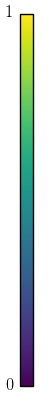
\includegraphics[height=5cm]{experiments/3d/vae_occ_sdf/colorbar_0}
%     %};
    
%     \node at (0, 1.2){
%       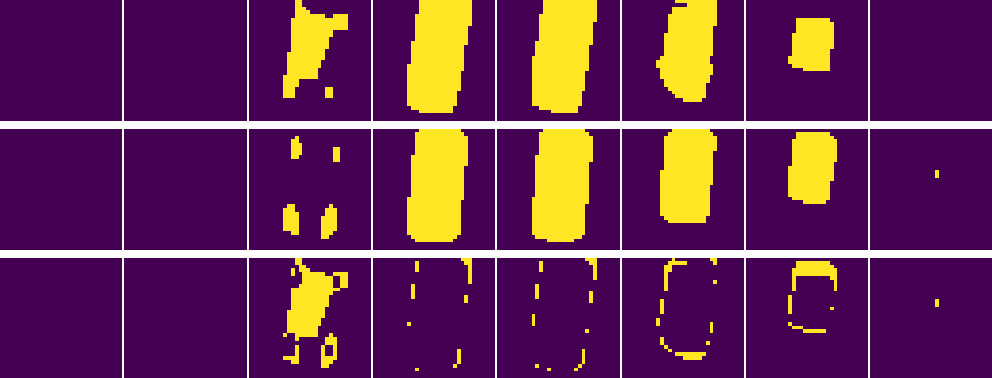
\includegraphics[width=6cm]{experiments/shapenet/vae_occ/easy_15_long/results_3}
%     };
%     \node at (0, -1.2){
%       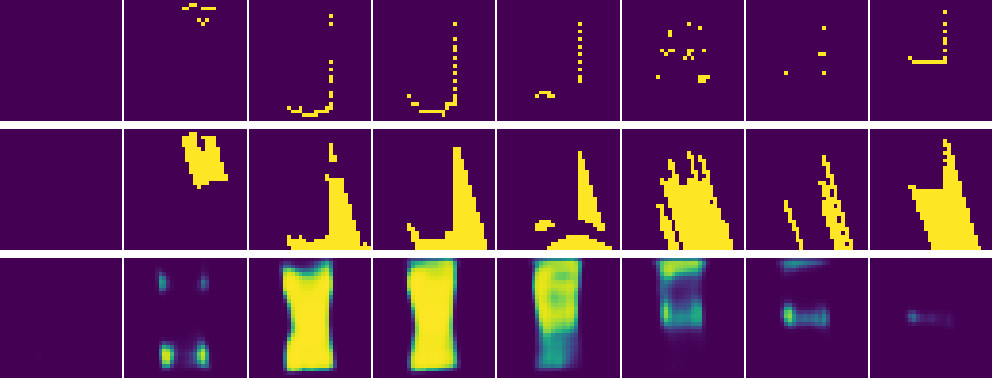
\includegraphics[width=6cm]{experiments/shapenet/vae_occ/easy_15_long/results_4}
%     };
    
%     \node at (6.5, 0){
%       \includegraphics[width=6cm]{experiments/shapenet/vae_occ/easy_15_long/random_1}
%     };
    
%     \node at (0, 3) {\begin{tabular}{c}reconstruction\\occupancy\end{tabular}};
%     \node at (6.5, 3) {\begin{tabular}{c}random samples\\occupancy\end{tabular}};
    
%     \draw[-,dashed] (-3.5, -2.5) -- (10, -2.5);
    
%     \node at (-3.5,-5) {
%       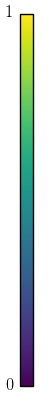
\includegraphics[height=5cm]{experiments/3d/vae_occ_sdf/colorbar_0}
%     };
    
%     \node at (0, -3.8){
%       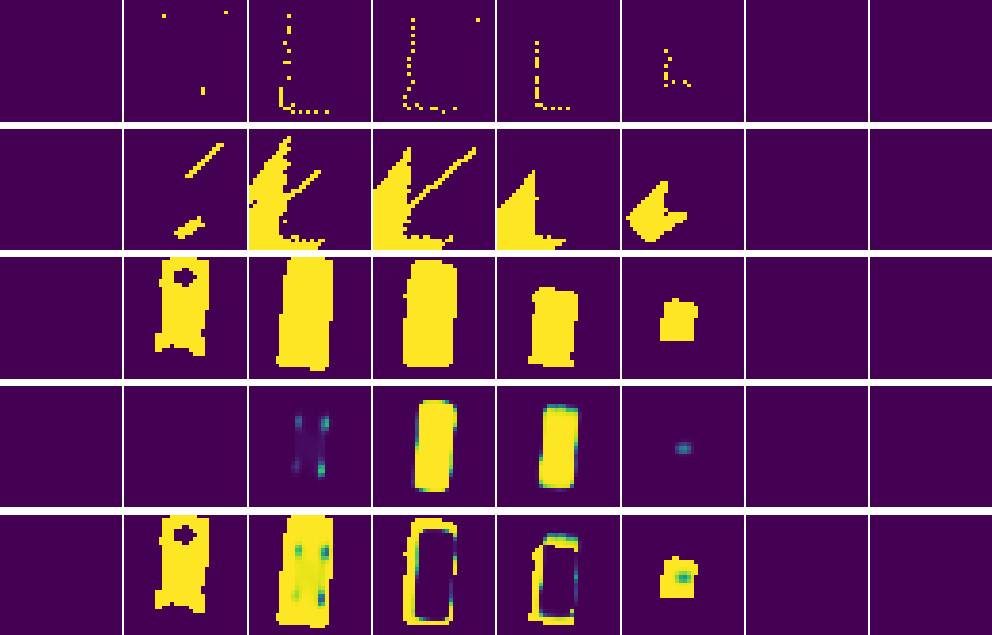
\includegraphics[width=6cm]{experiments/shapenet/vae_occ_sdf/easy_15/results_0_0}
%     };
%     \node at (0, -6.2){
%       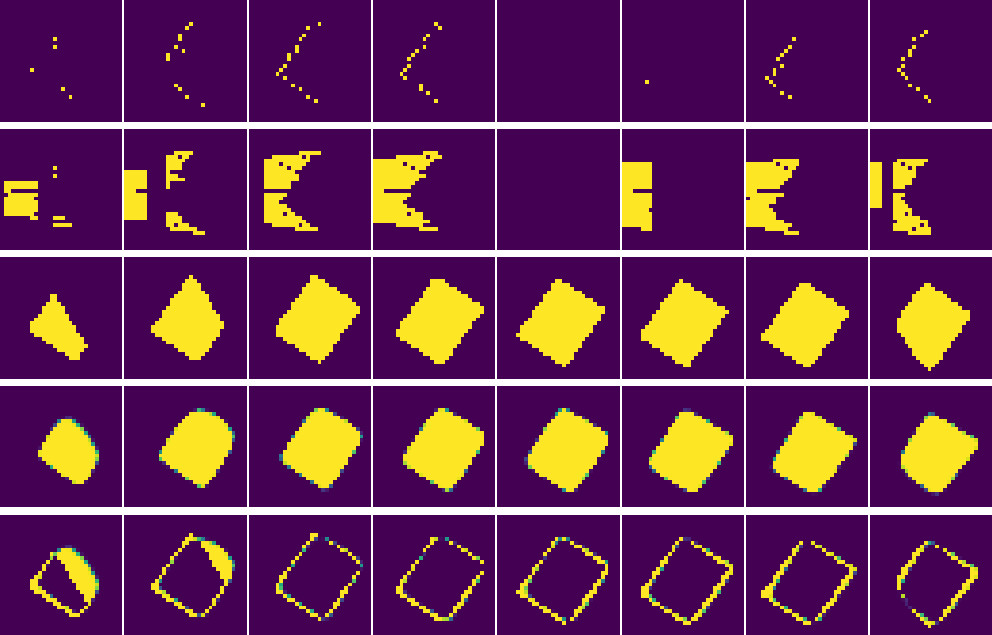
\includegraphics[width=6cm]{experiments/shapenet/vae_occ_sdf/easy_15/results_1_0}
%     };
%     \node at (0, -9.75){
%       \includegraphics[width=6cm]{experiments/shapenet/vae_occ_sdf/easy_15/random_1_0}
%     };
    
%     %\draw[-,dashed] (3.25, -3) -- (3.25,3);
    
%     \node at (6.5, -3.8){
%       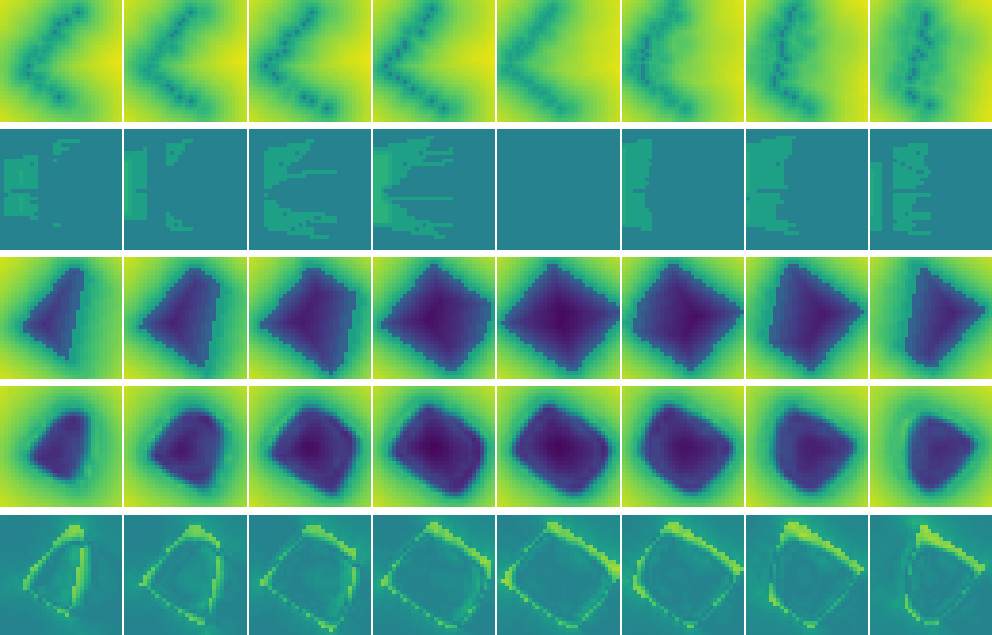
\includegraphics[width=6cm]{experiments/shapenet/vae_occ_sdf/easy_15/results_0_1}
%     };
%     \node at (6.5, -6.2){
%       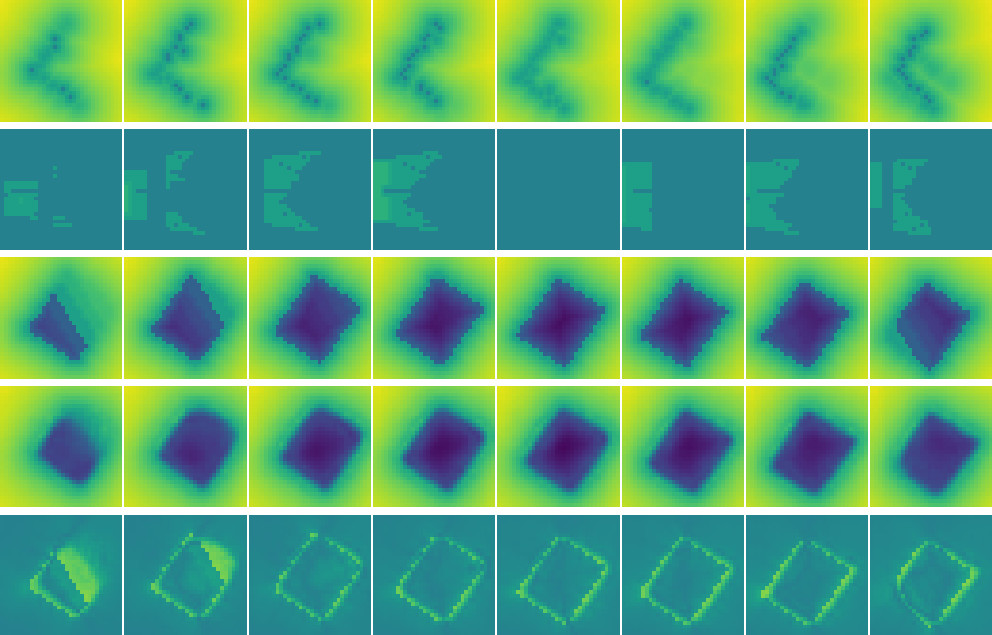
\includegraphics[width=6cm]{experiments/shapenet/vae_occ_sdf/easy_15/results_1_1}
%     };
%     \node at (6.5, -9.75){
%       \includegraphics[width=6cm]{experiments/shapenet/vae_occ_sdf/easy_15/random_1_1}
%     };
    
%     \node at (10,-5) {
%       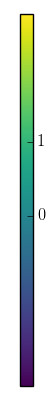
\includegraphics[height=5cm]{experiments/3d/vae_occ_sdf/colorbar_1}
%     };
    
%     \node at (0, -13) {\begin{tabular}{c}reconstruction\\random samples\\occupancy\end{tabular}};
%     \node at (6.5, -13) {\begin{tabular}{c}reconstruction\\random samples\\signed distance functions\end{tabular}};
%   \end{tikzpicture}
%   \caption{Qualitative results corresponding to reconstruction and random
%   samples for two \VAE models with $Q = 15$: first, trained on occupancy only (top),
%   second trained on both occupancy and signed distance functions (bottom). For
%   illustrating reconstruction performance, we show horizontal slices of the volumes
%   corresponding to the observed points, partial free space, target shape as well
%   as predicted shape and the corresponding error. 3D visualizations corresponding
%   to the shown random samples can be found in Figures
%   \ref{fig:appendix-experiments-shapenet-vae-qual-3} and
%   \ref{fig:appendix-experiments-shapenet-vae-qual-4}. For reconstruction,
%   we present 3D visualizations in Figure \ref{fig:appendix-experiments-shapenet-vae-qual-2}.}
%   \label{fig:appendix-experiments-shapenet-vae-qual-1}
% \end{figure}
\begin{figure}[h]
  \centering
  \begin{subfigure}[t]{1\textwidth}
    \hspace*{-0.75cm}
    \begin{tikzpicture}
      \node at (0, 0) {
        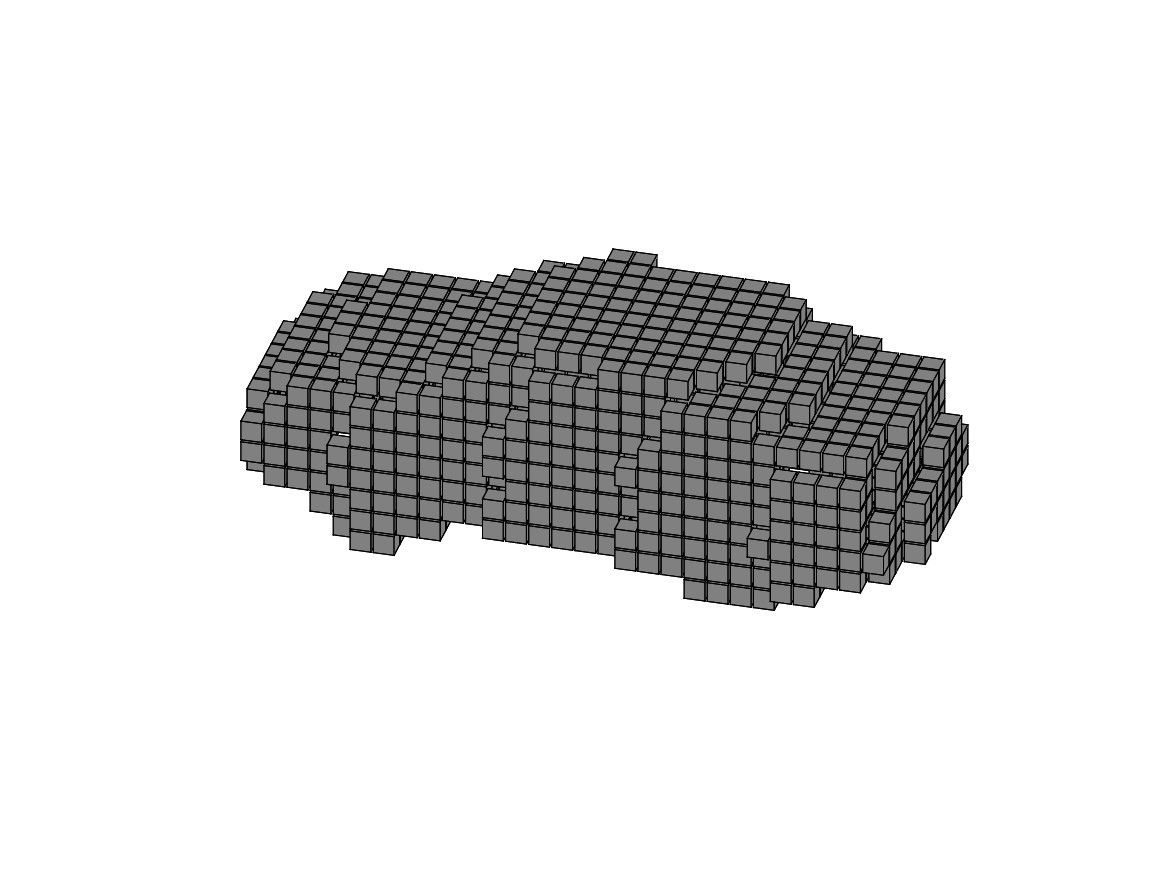
\includegraphics[width=2.5cm,trim={2cm 1cm 2cm 1cm},clip]{experiments/shapenet/vae_occ/easy_15_long/0_target_15}
      };
      \node at (2.5, 0) {
        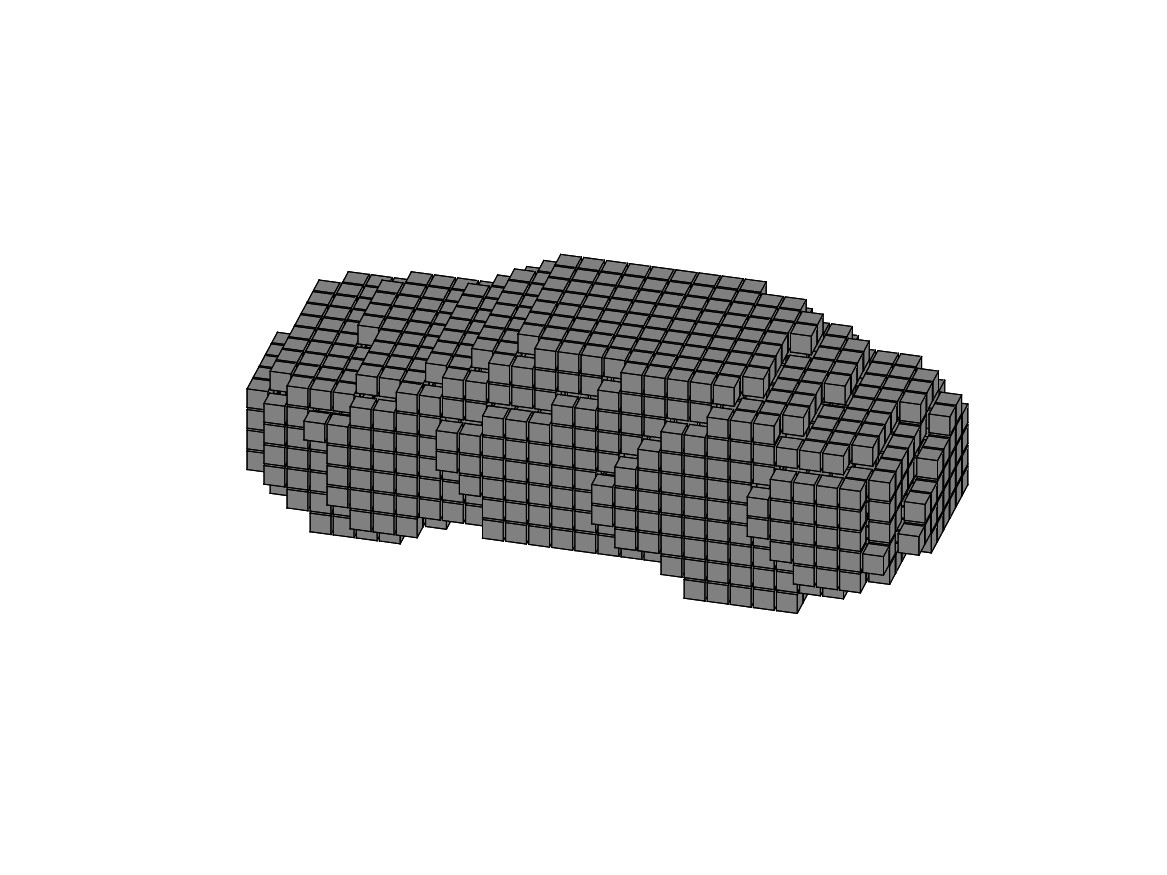
\includegraphics[width=2.5cm,trim={2cm 1cm 2cm 1cm},clip]{experiments/shapenet/vae_occ/easy_15_long/0_prediction_15}
      };
      \node at (5, 0) {
        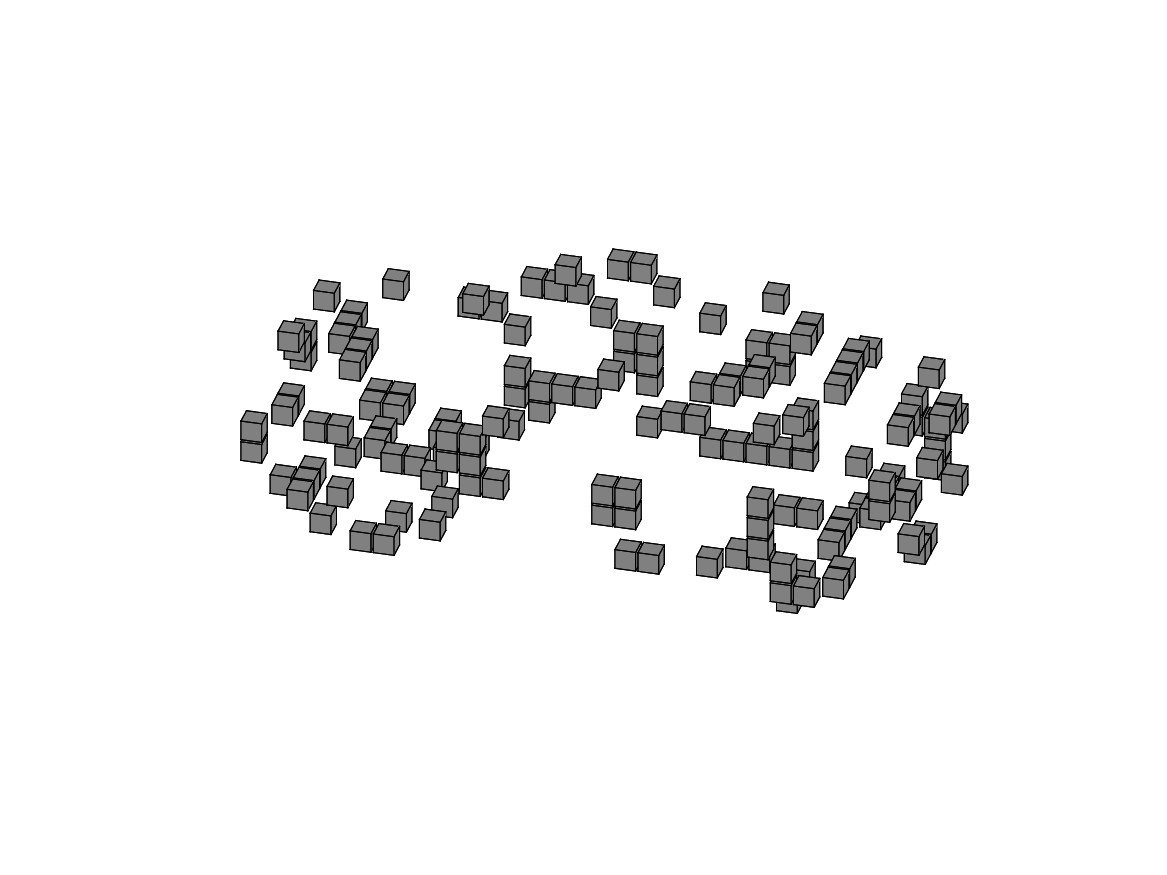
\includegraphics[width=2.5cm,trim={2cm 1cm 2cm 1cm},clip]{experiments/shapenet/vae_occ/easy_15_long/0_error_15}
      };
      
      \draw[-,dashed] (6.375,-1) -- (6.375, 1);
      
      \node at (8, 0) {
        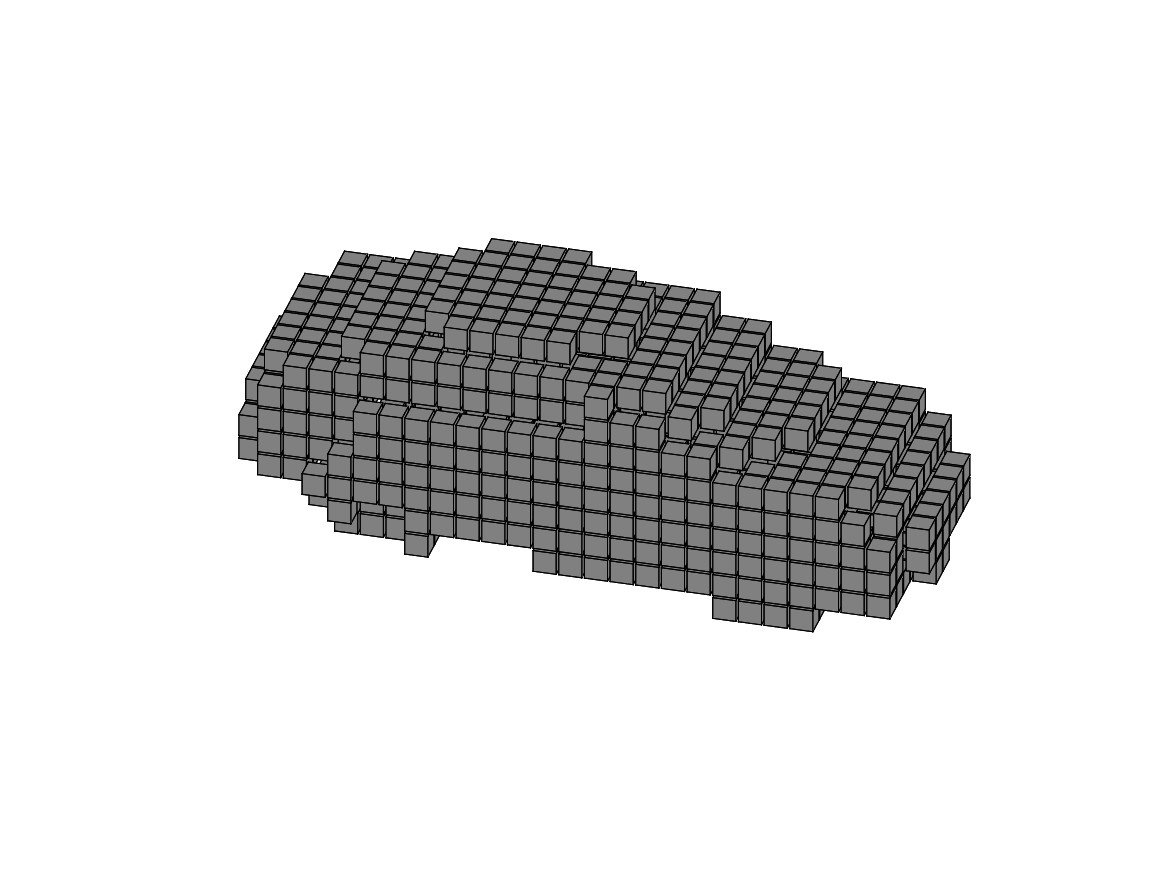
\includegraphics[width=2.5cm,trim={2cm 1cm 2cm 1cm},clip]{experiments/shapenet/vae_occ/easy_15_long/1_target_15}
      };
      \node at (10.5, 0) {
        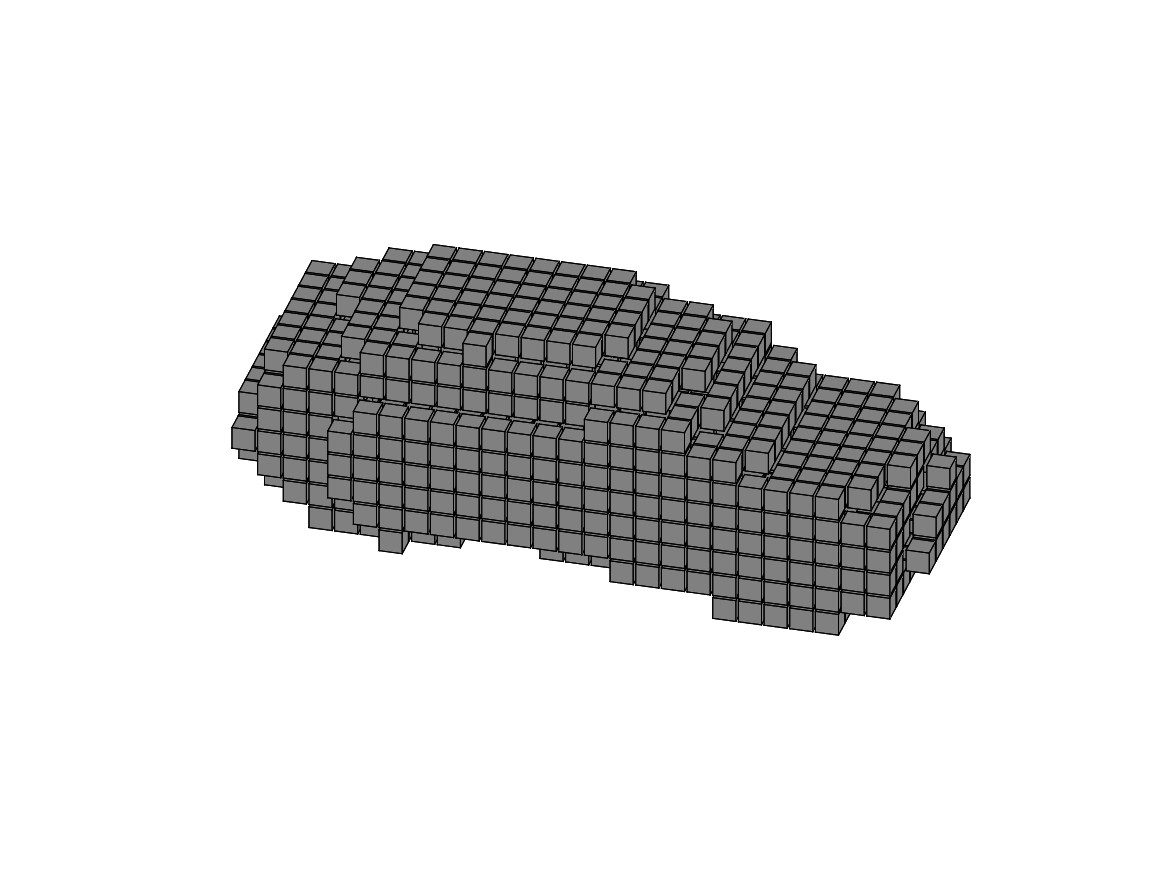
\includegraphics[width=2.5cm,trim={2cm 1cm 2cm 1cm},clip]{experiments/shapenet/vae_occ/easy_15_long/1_prediction_15}
      };
      \node at (13, 0) {
        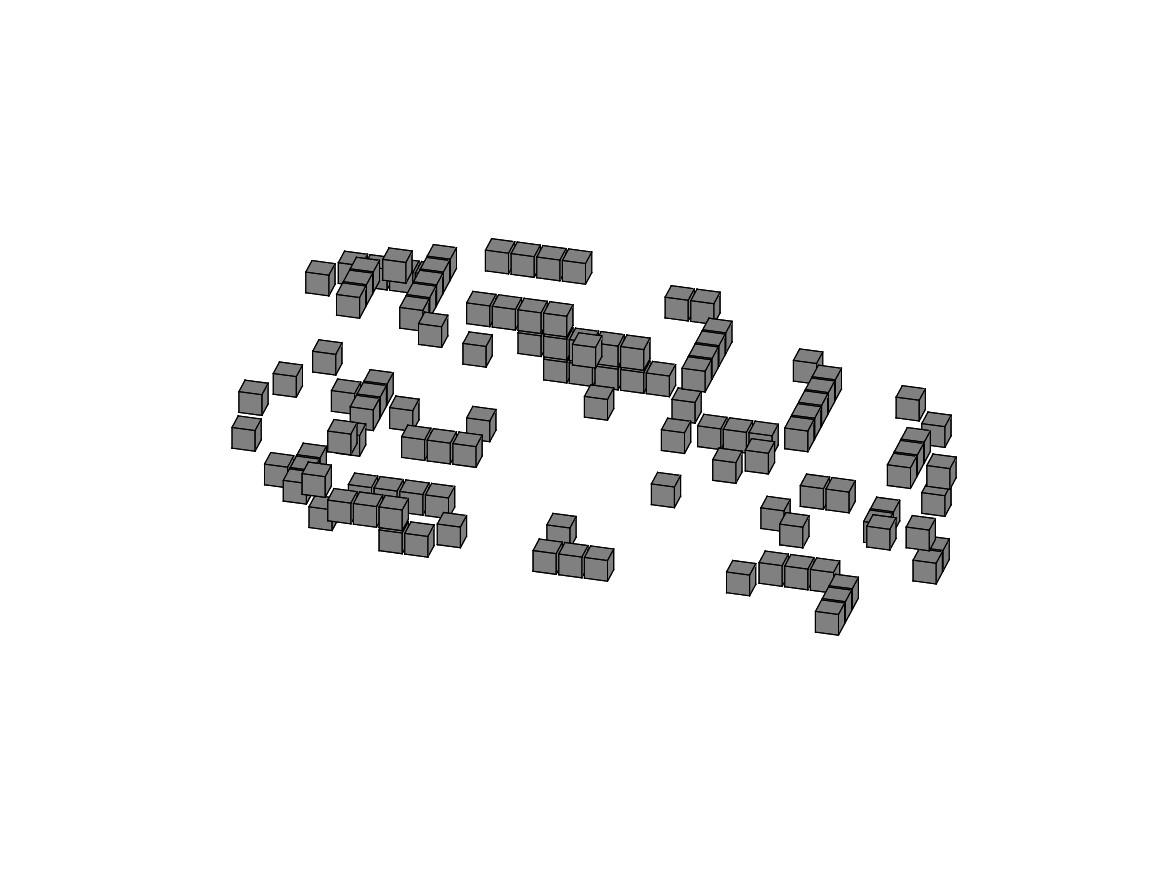
\includegraphics[width=2.5cm,trim={2cm 1cm 2cm 1cm},clip]{experiments/shapenet/vae_occ/easy_15_long/1_error_15}
      };
      
      \node at (0, 1) {Target};
      \node at (2.5, 1) {Reconstruction};
      \node at (5, 1) {Error};
      
      \node at (8, 1) {Target};
      \node at (10.5, 1) {Reconstruction};
      \node at (13, 1) {Error};
    \end{tikzpicture}
    \subcaption{3D visualizations of the reconstruction capabilities using occupancy only. We show
    the occupancy grids corresponding to the target shape, the reconstructed shape and its error.}
    \label{fig:appendix-experiments-shapenet-vae-qual-2}
  \end{subfigure}\\[10px]
  \begin{subfigure}[t]{1\textwidth}
    \hspace*{-0.75cm}
    \begin{tikzpicture}
      \node at (0, 0) {
        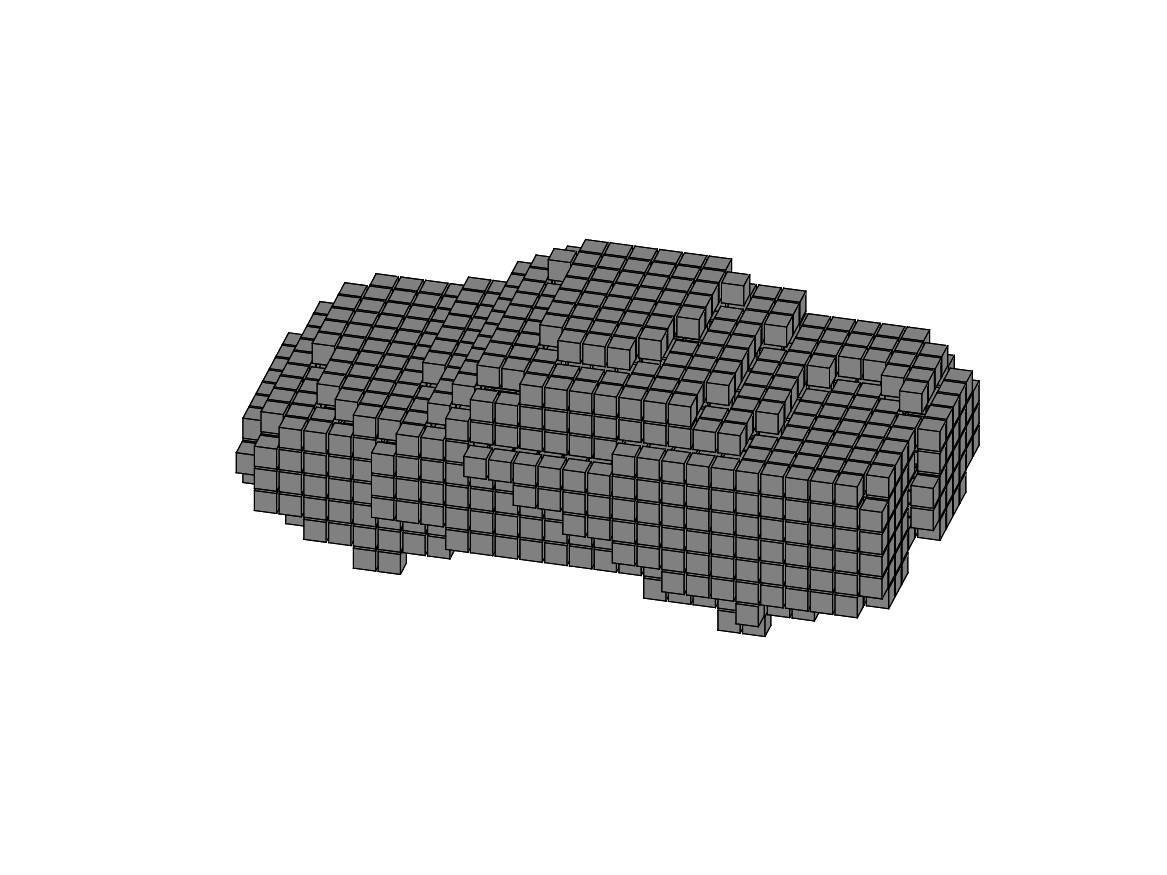
\includegraphics[width=2.5cm,trim={2cm 1cm 2cm 1cm},clip]{experiments/shapenet/vae_occ/easy_15_long/1_random_15}
      };
      \node at (2.5, 0) {
        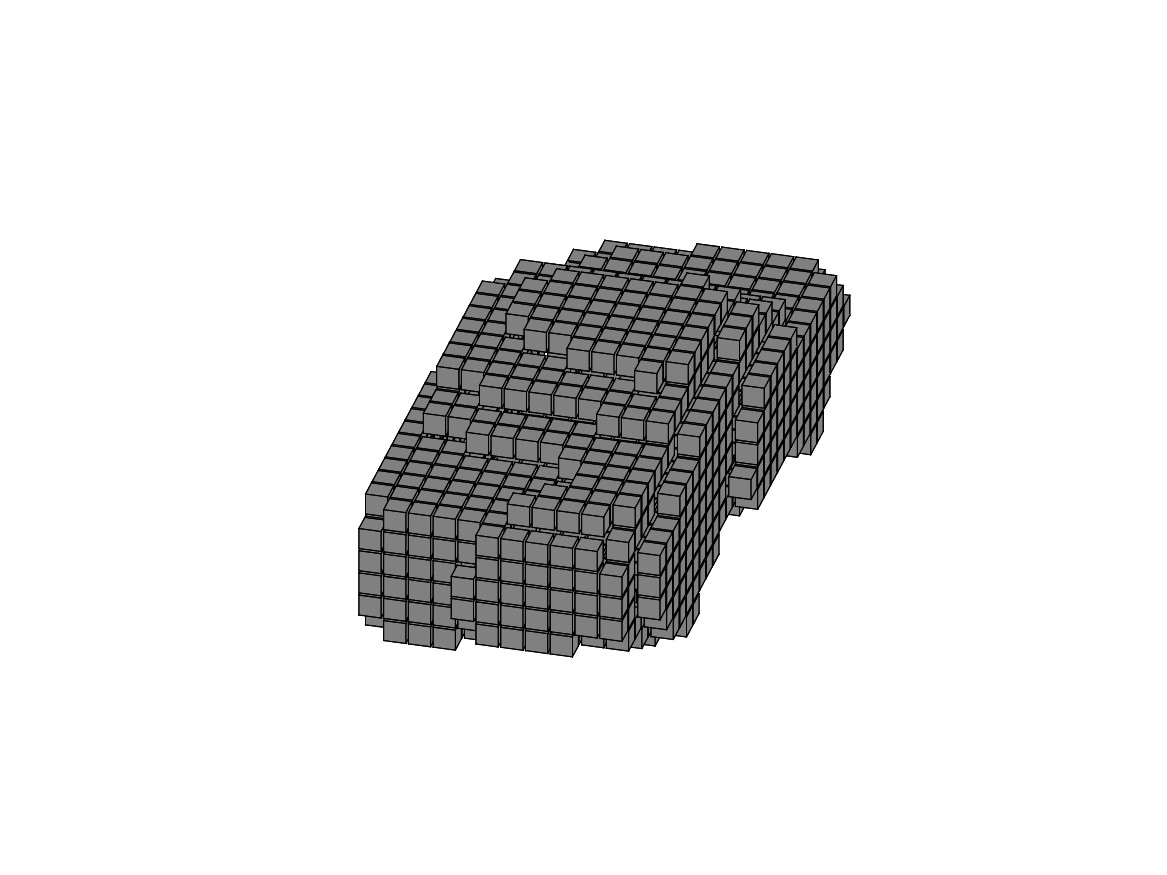
\includegraphics[width=2.5cm,trim={2cm 1cm 2cm 1cm},clip]{experiments/shapenet/vae_occ/easy_15_long/1_random_105}
      };
      
      \draw[-,dashed] (4,-1) -- (4, 1);
      
      \node at (5.5, 0) {
        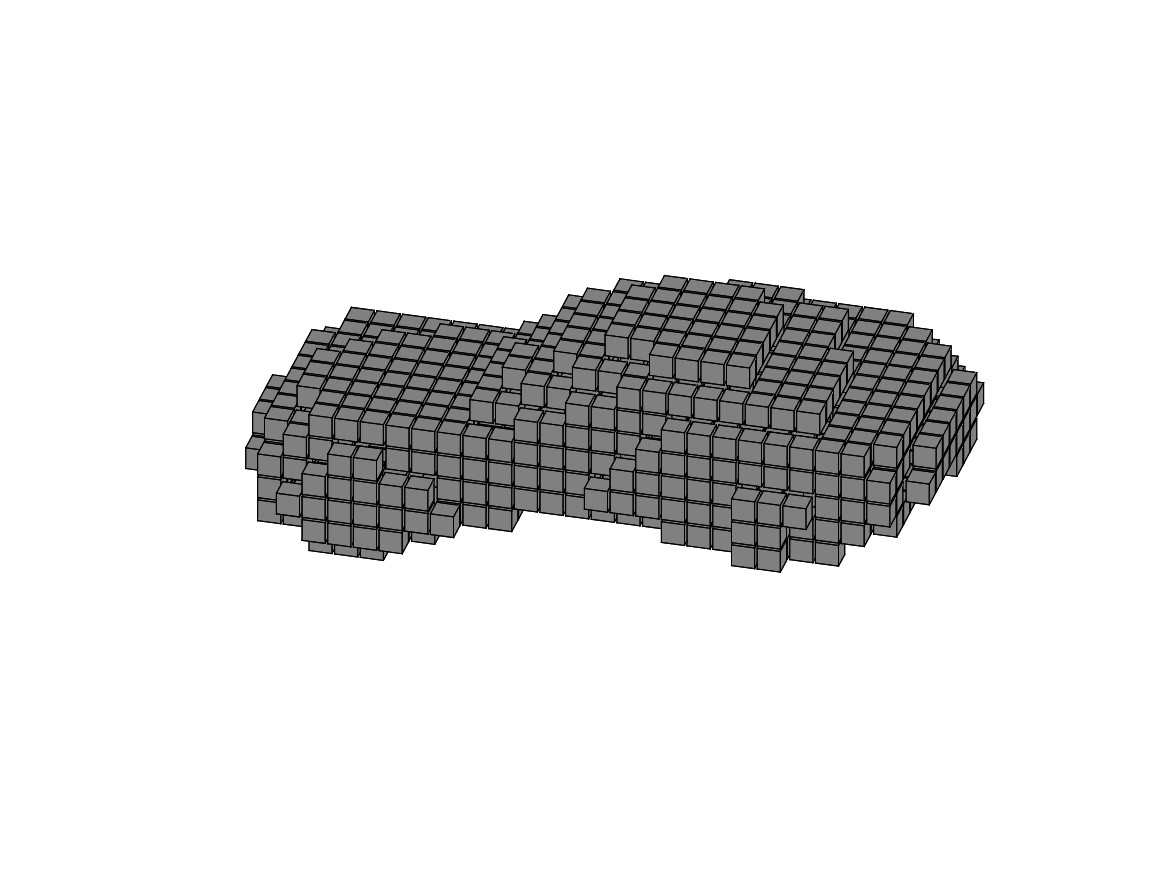
\includegraphics[width=2.5cm,trim={2cm 1cm 2cm 1cm},clip]{experiments/shapenet/vae_occ/easy_15_long/6_random_15}
      };
      \node at (8, 0) {
        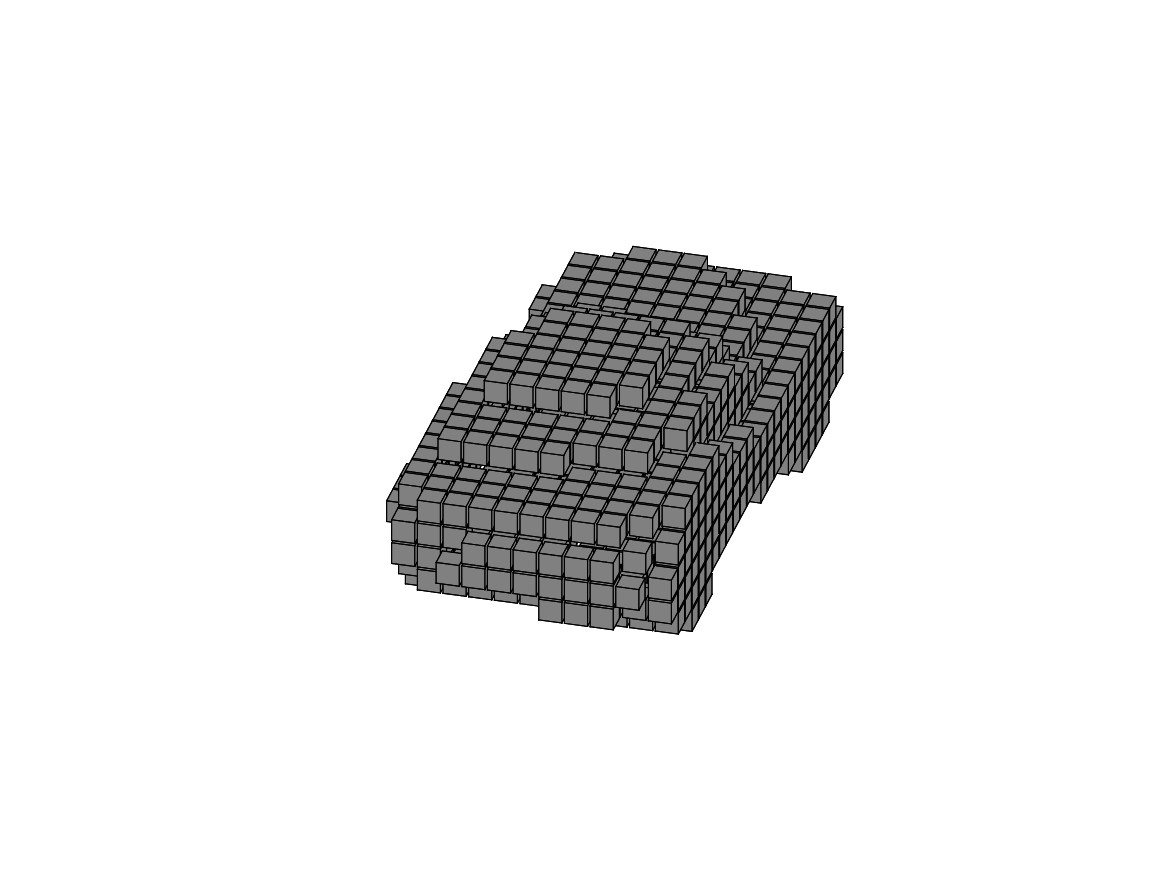
\includegraphics[width=2.5cm,trim={2cm 1cm 2cm 1cm},clip]{experiments/shapenet/vae_occ/easy_15_long/6_random_105}
      };
      
      \draw[-,dashed] (9.5,-1) -- (9.5, 1);
      
      \node at (11, 0) {
        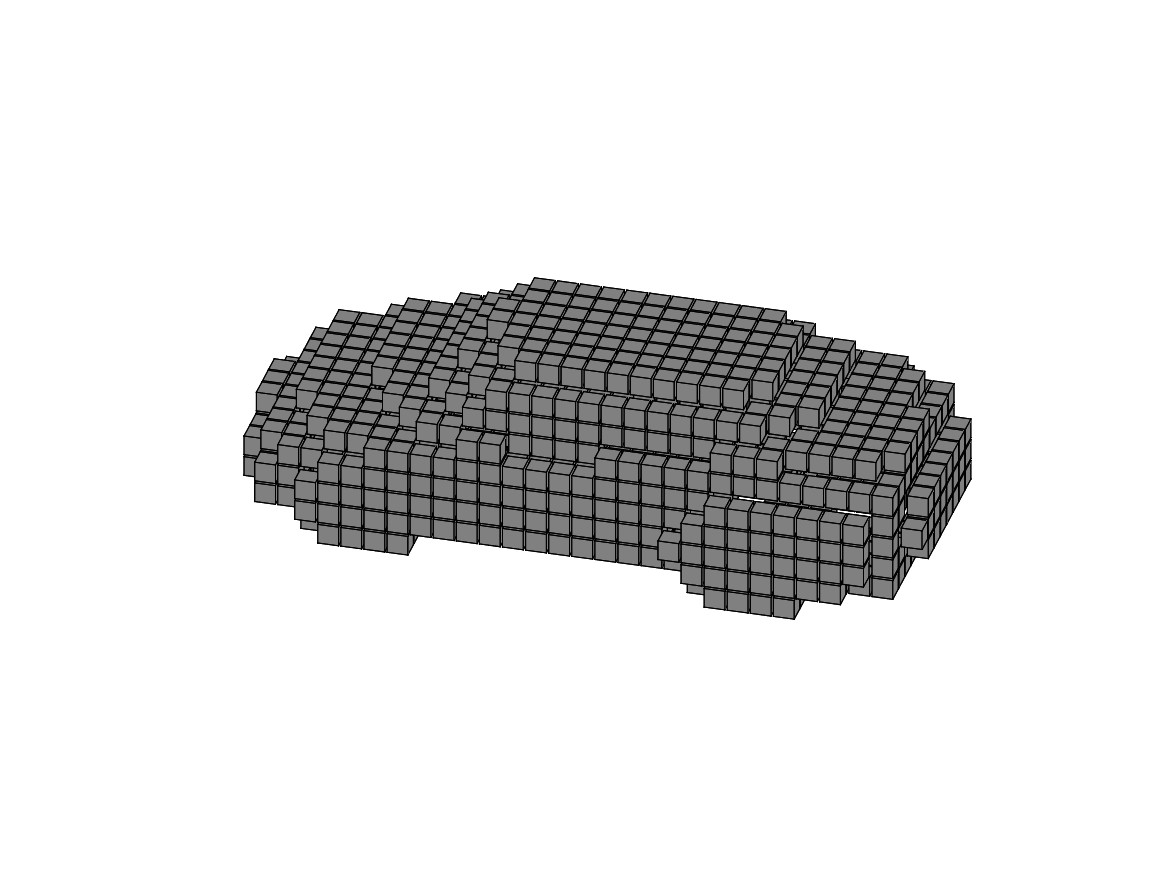
\includegraphics[width=2.5cm,trim={2cm 1cm 2cm 1cm},clip]{experiments/shapenet/vae_occ/easy_15_long/7_random_15}
      };
      \node at (13.5, 0) {
        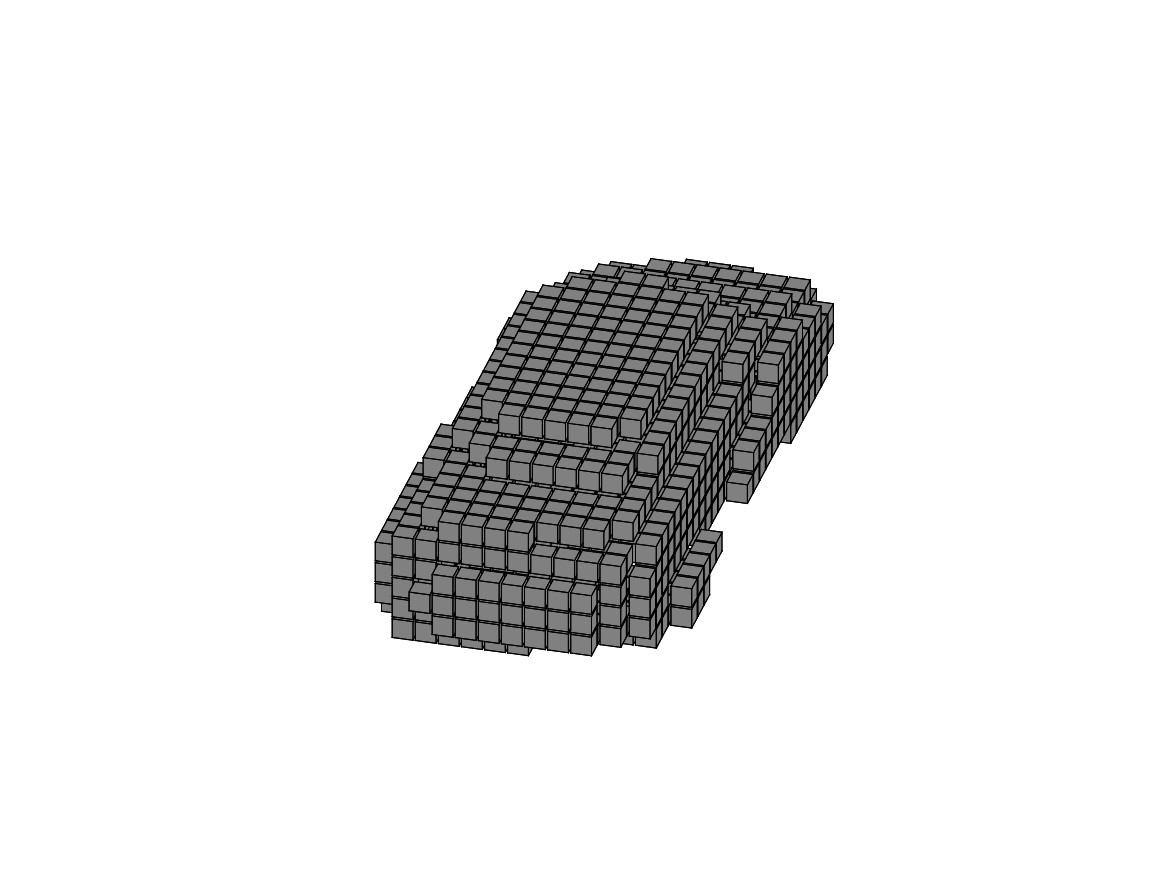
\includegraphics[width=2.5cm,trim={2cm 1cm 2cm 1cm},clip]{experiments/shapenet/vae_occ/easy_15_long/7_random_105}
      };
    \end{tikzpicture}
    \subcaption{3D visualizations of random samples generated in the occupancy only case.
    Each sample is shown from two distinct viewpoints.}
    \label{fig:appendix-experiments-shapenet-vae-qual-3}
  \end{subfigure}\\[14px]
  \begin{subfigure}[t]{1\textwidth}
    \hspace*{-0.25cm}
    \begin{tikzpicture}   
      \node at (0, 0) {
        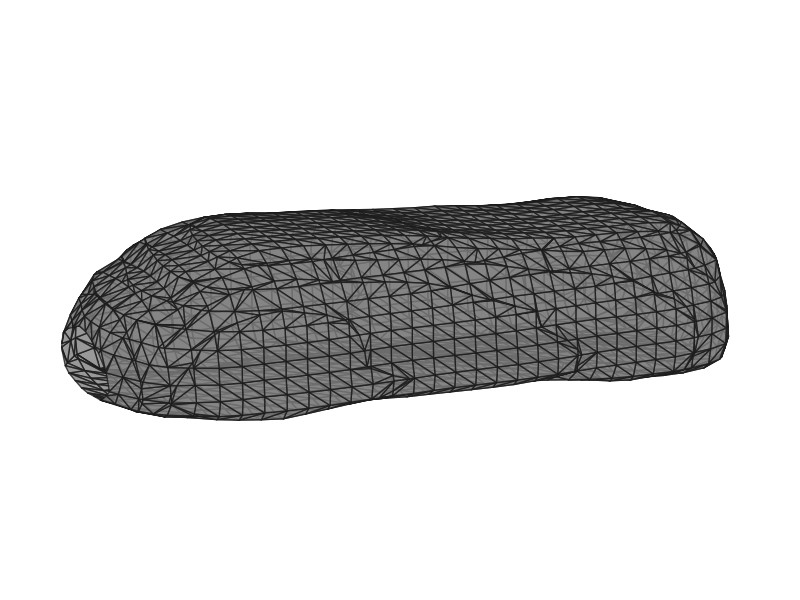
\includegraphics[width=2.4cm,trim={1cm 3cm 1cm 3cm},clip]{experiments/shapenet/vae_occ_sdf/easy_15/6_random}
      };
      
      \draw[-,dashed] (1.25,-1) -- (1.25, 1);
      
      \node at (2.5, 0) {
        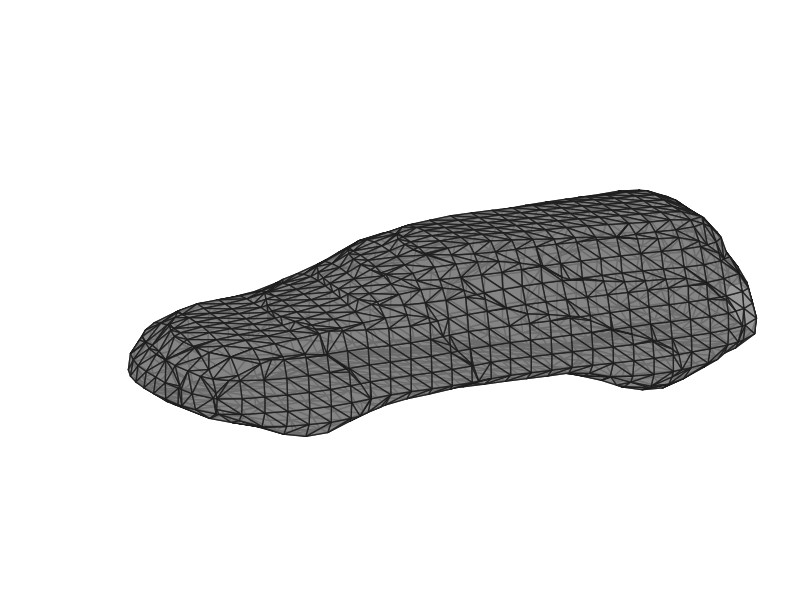
\includegraphics[width=2.4cm,trim={1cm 3cm 1cm 3cm},clip]{experiments/shapenet/vae_occ_sdf/easy_15/7_random}
      };
      
      \draw[-,dashed] (3.75,-1) -- (3.75, 1);
      
      \node at (5, 0) {
        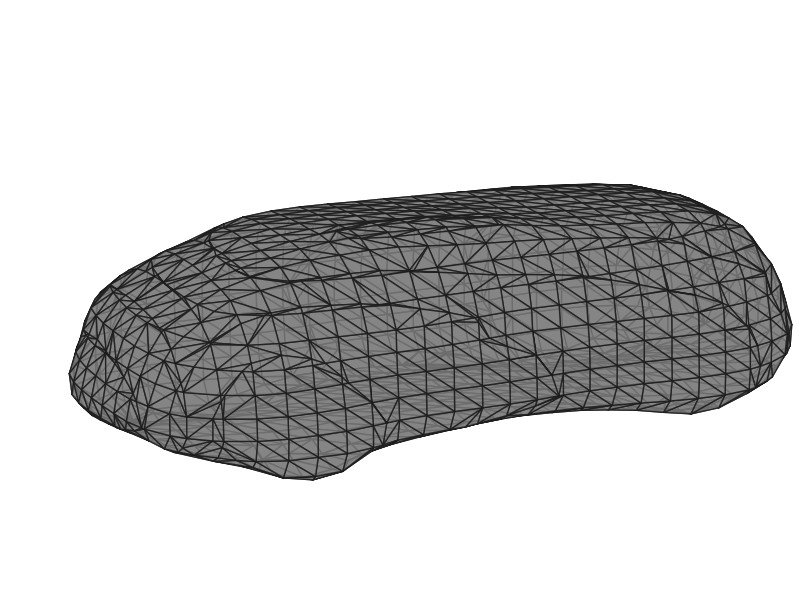
\includegraphics[width=2.4cm,trim={1cm 3cm 1cm 3cm},clip]{experiments/shapenet/vae_occ_sdf/easy_15/8_random}
      };
      
      \draw[-,dashed] (6.25,-1) -- (6.25, 1);
      
      \node at (7.5, 0) {
        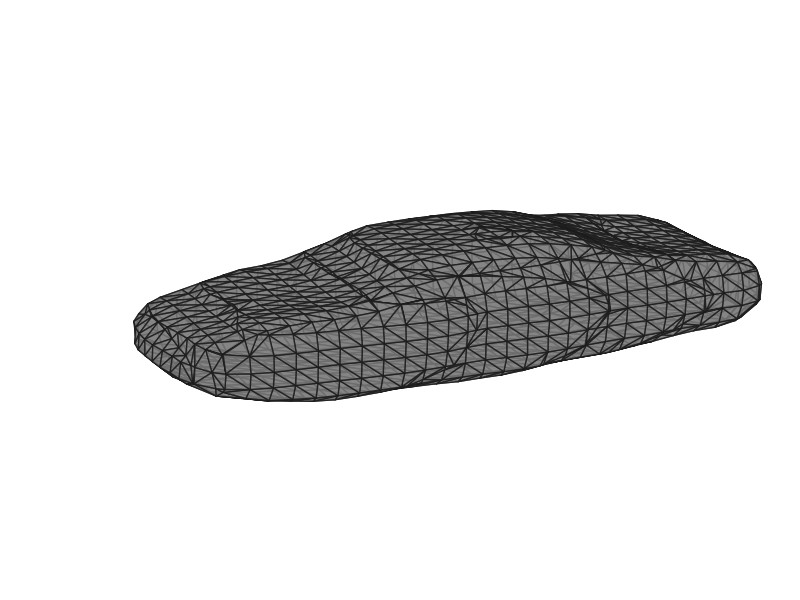
\includegraphics[width=2.4cm,trim={1cm 3cm 1cm 3cm},clip]{experiments/shapenet/vae_occ_sdf/easy_15/9_random}
      };
      
      \draw[-,dashed] (8.75,-1) -- (8.75, 1);
      
      \node at (10, 0) {
        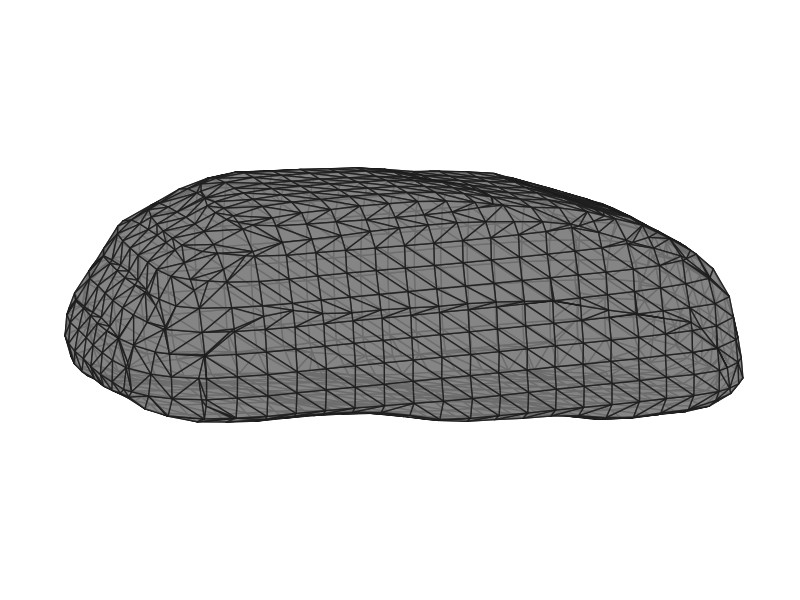
\includegraphics[width=2.4cm,trim={1cm 3cm 1cm 3cm},clip]{experiments/shapenet/vae_occ_sdf/easy_15/10_random}
      };
      
      \draw[-,dashed] (11.25,-1) -- (11.25, 1);
      
      \node at (12.5, 0) {
        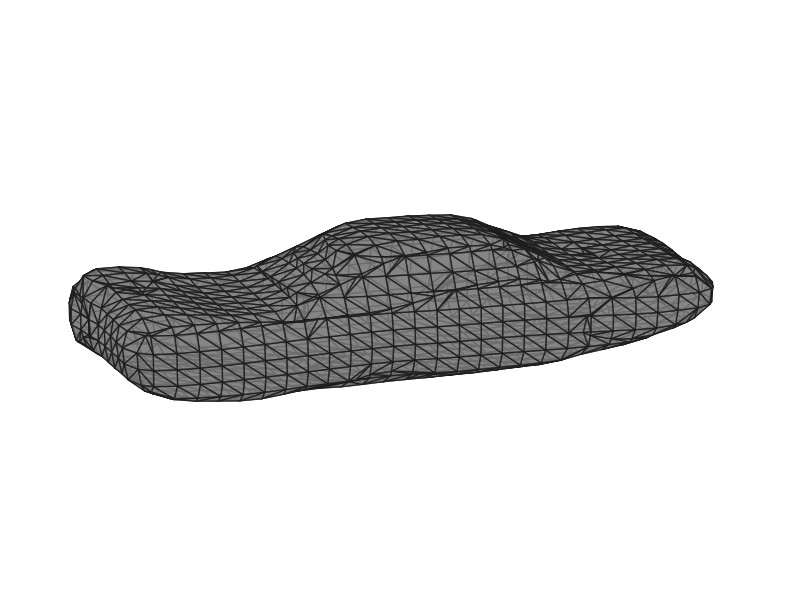
\includegraphics[width=2.4cm,trim={1cm 3cm 1cm 3cm},clip]{experiments/shapenet/vae_occ_sdf/easy_15/11_random}
      };
    \end{tikzpicture}
    \subcaption{Random samples generated using both occupancy and signed distance functions,
     We show meshes obtained by
    running marching cubes \cite{LorensenCline:1987} on the generated
    signed distance functions.}
    \label{fig:appendix-experiments-shapenet-vae-qual-4}
  \end{subfigure}
  \vskip 6px
  \caption{Additional qualitative results for a \VAE shape prior using $Q = 15$ trained on
  occupancy only, Figures \ref{fig:appendix-experiments-shapenet-vae-qual-2}
  and \ref{fig:appendix-experiments-shapenet-vae-qual-3}, and on both modalities,
  Figure \ref{fig:appendix-experiments-shapenet-vae-qual-4}, using ShapeNet.}
  \label{fig:appendix-experiments-vae-qual}
\end{figure}